%------------------------------------------------------------------
%
% Vorlage für Abschlussarbeiten an der Technischen Hochschule Ingolstadt
% Bachelorarbeit/Masterarbeit
%
% Angepasst auf Seminararbeit
%
% V1 05.12.2011		Dr. Paul Spannaus
% V2 07.07.2012		Dr. Paul Spannaus
% V3 10.03.2013		Dr. Paul Spannaus
% V4 28.01.2014		Dr. Paul Spannaus
% V5 31.10.2014 		Dominik Schlecht
% 	
% -----------------------------------------------------------------
% -----------------------------------------------------------------

% Dokumentenklasse
\documentclass[a4paper,11pt,DIV=11,oneside]{scrreprt} % 

% Packages
%Datum und Uhrzeit
\usepackage{datetime}

%Encoding
\usepackage[utf8]{inputenc}
\usepackage{lmodern}

%Graphikpakete
\usepackage{graphicx}
\usepackage{xcolor}
\usepackage{tikz}
\usetikzlibrary{arrows, snakes, backgrounds}
\usepackage{wrapfig}

% Farben der THI
\definecolor{THIblue}{rgb}{0.0078,0.1176,0.4705}

\usepackage[ngerman]{babel}

%Zitierumgebung
%\usepackage{cite}% Zitieren
\usepackage[backend=biber,]{biblatex}
%\usepackage{bibgerm}% Literatur in Deutscher DIN
\usepackage[babel,german=quotes]{csquotes}

%%-------------Silbentrennung--------------------------------------
\hyphenation{}

%%-------------Index-----------------------------------------------
%\makeindex

%------------------------------------------------------------------
% Angabe der zu verwendenden Dateien, sodass nur z.B. das aktuelle 
% Dokument compiliert wird; den Rest mit % auskommentieren
\includeonly{
    chapter/Intro,
    chapter/Setup,
    chapter/Dungeon,
}

%-----------------------------------------------------------------
%---------------Dokumentenbeginn----------------------------------
%-----------------------------------------------------------------
\begin{document}
	\pagenumbering{roman} % Nummerierung
%---------------Hauptteil-----------------------------------------
	\pagenumbering{arabic} 	% Neunummerierung des Hauptteils
	\setcounter{page}{1}	% Wieder bei 1 Anfangen
	
	%intro
	\chapter{Intro}
Der iCTF (international Capture The Flag) wird jährlich von der University of California, Santa Barbara veranstaltet und ist der größten Hackerwettbewerbe dieser Art. 
Der iCTF integriert Angriff und Verteidigung zugleich. Die Teilnehmer müssen gleichzeitig Flaggen von fremden Servicen klauen, sowie ihre eigenen Service patchen um diese unangreifbar zu machen. 
Dieses Jahr fand der Wettbewerb am 04.12. statt und ca. 40 Teams nahmen daran Teil. Dabei belegte unser Team (in23canation) den 22. Platz. Die Dauer des Wettbewerbs wurde mit 24 Stunden angekündigt jedoch kurz vor dem iCTF auf 8 Stunden reduziert. 
Die Stimmung beim Wettbewerb war durchgehend positiv und insgesamt war der CTF ein großer Erfolg. Durch etwas Werbung vorab war es möglich eine große Teilnehmerzahl aus allen Semestern zu begeistern sich unserer Gruppe anzuschließen. Schon bei den zwei vorangehenden Informationsveranstaltungen waren ungefähr 60 Studenten anwesend. Beim iCTF selber waren rund 25 Teilnehmer aktiv dabei. 
	
		\section{Network-Setup}
	The setup of the iCTF 2015 is shown in the graphic \ref{img:setup}. The Router has a private VPN running, tunneling all traffic through the THI-Network. Also the Router creates 2 sub-networks. The "bad network" (shown in red) holds the iCTF-Router and vulnerable VM, as well as some attacker PCs, which will run the exploits against other teams. In the "good network" (shown in green) are the participants, who have a local copy of the vulnerable Image and develop patches and exploit. It's to mention, that the router has ip-tables-rules specified, so the "bad network" can not communicate with the "good network". Also, the Attacker-PCs have to route their traffic through the CTF-Router. This should be solved differently in the upcoming CTFs, since the separation of the 2 networks needed a lot of time to be configured.
	\begin{figure}
		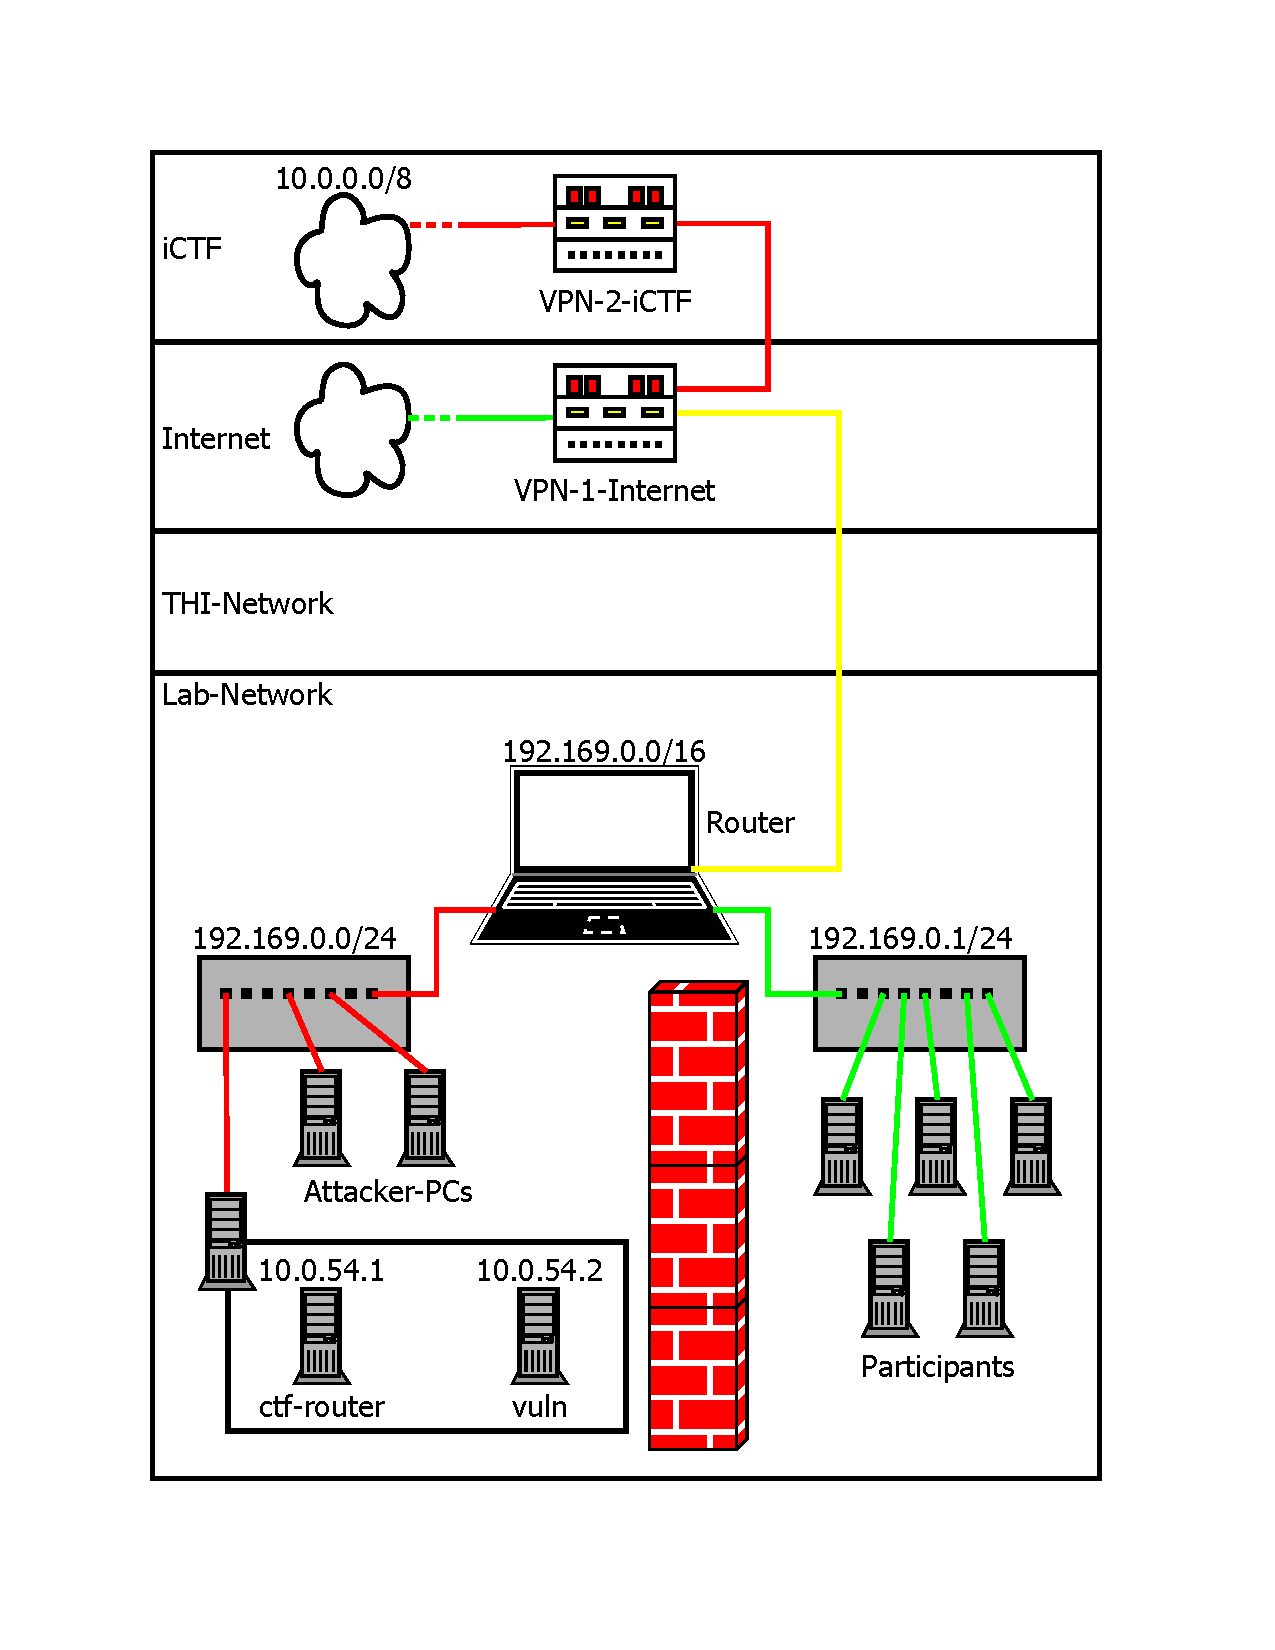
\includegraphics[width=\textwidth]{images/setup.pdf}
		\caption{Network-Setup iCTF 2015}
	\end{figure}
	%Dungeon Service
	\label{img:setup}
	\chapter{Dungeon}


\section{Aufbau und Configuration}


\section{Services: Dungeon}
The Dungeon service was a consoleservice which presented a litte game. The player needs to run through the dungeon to finally kill a dragon in the end. To do this, two items are needed. Firstly a golden sabre and second a magic shield. If either of the items is missing the player will die to the dragon.
To get the sabre the player needs to find a secret room and in there has to get the name of an airplane picture right. If he does he will get the sabre. 
Now the player will get in a room with a dwarf. He says if you get the number i guess you will get my shield. But the number he has is random generated and nearly impossible to get right. Also if you get the number right he will tell you that he gives you the shield but the variable HAVE\_SHIELD will not change. To achive the shield the player has to go to a room with a gnome which asks the player's name and then says Hi! playername. In this function there is an adress returned with the variable HAVE\_SHIELD. So the player need to type in anycharacter than \%n so that the adress will be overwritten with 0x1.
If the player encounters the dragon with both items he can slay the dragon with the command "'kill dragon"'. After that he will be asked what his name is. Here comes the tricky part. With a Bufferoverflow it is possible to alter the return adress so that the function will jump to the secret treasure room where the flag can be optained. To do this the player have to type 88 random characters followed by 0xDEADBEEF in ASCII than 8 random characters again and then the adress to the storage room. The 0xDEADBEEF is needed because a value is checked for change. If you overwrite it with the bufferoverflow the service will disconnect the player. Both 0xDEADBEEF and the return adress have to be turned because little Endian is used. 


%Der Dungeon Service war ein Consolenservice der ein Spiel darstellt. der Spieler muss dabei durch ein Dungeon laufen und am Ende einen Drachen töten. Um dies zu bewerkstelligen werden 2 Gegenstände gebraucht. Ein goldener Säbel und ein magisches Schild. 
%Um den Säbel zu bekommen muss zuerst ein geheimer Raum gefunden werden in dem der Namen eines Flugzeuges anhand eines Abbilds erraten werden muss. Wird richtig geraten erhält der Spieler den Säbel. 
%Des weiteren gibt es einen Raum, bei dem ein Zwerg sein Schild abgibt, wenn du seine Nummer errätst. Dies ist jedoch fast unmöglich da die Nummer zufällig bestimmt wird. Des weiteren bekommt man den Schild ebenfalls nicht wenn man die Nummer errät. 
%Um diesen nun zu bekommen muss in einem anderen Raum bei einem Gnom der nach den Spielernamen fragt den Speicher überschreiben. Die Funktion übergibt die Adresse der Variable HAVE\_SHIELD und wenn man ein beliebiges Zeichen und dann \%n eingibt, wird auf der Adresse HAVE\_SCHIELD eine 1 eingetragen. 
%Wenn der Spieler nun beim Drachen ist, stirbt er nicht wie sonst, sondern kann den Drachen mit dem command  "'kill dragon"' töten. 
%Im Anschluss daran wird er Spieler erneut nach seinem Namen gefragt. Nun kann man mithilfe eines Bufferoverflows die Rücksprungadresse der Funktion so ändern, dass der Spieler im Secret Storage Room landet. Dort wird die Flagge ausgegeben, wenn die ID angegeben wird. Eine Hürde beim Bufferoverflow ist jedoch, dass auf eine Variable geprüft wird und wenn die überschrieben wird, wird der Nutzer vom Service getrennt. Um dies zu verhindern muss genau ab der 88. Stelle 0xDEADBEEF in ASCII mitübergeben werden. Danach noch 4 Zufallszeichen und dann die Rücksprungadressse. 0xDEADBEEF sowie die Rücksprungadresse müssen umgedreht werden, das litte Endian verwendet wird.
	
%---------------Anhang-------------------------------------------
	%
%------------------------------------------------------------------------
% Anhänge
\appendix
\chapter{Appendix}
\section{Quellcode}
\section{Ergänzende Grafiken}
\section{Quellcode Grafiken}
 % Anhang
	%\newpage
	%\printbibliography % Literaturliste
\end{document}
%-----------------------------------------------------------------
%---------------Dokumentenende------------------------------------
%-----------------------------------------------------------------
